% Drop-in for S4.3, next to the retrieval result. Requires:
%   cp DanielNewWork/figures/copying.pdf paper/figures/
% Every number below is figure-local (conditioning graph val. #0 and the two
% index-0 samples) and is printed by DanielNewWork/make_copying_figure.py.
% It deliberately quotes no population mean -- see DanielNewWork/README.md on
% the matched-F1 discrepancy -- and points at S4.3 for the 32-graph result.

\begin{figure}[t]
\centering
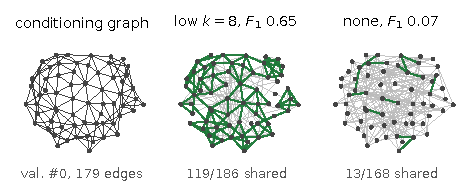
\includegraphics[width=\columnwidth]{figures/copying.pdf}
\caption{The copying, on one graph. All three panels use a single layout
computed on the conditioning graph, so an edge a sample shares with it is drawn
in the same place in both panels: \textcolor[HTML]{1b7837}{green} edges are
shared, grey are not. The \texttt{low} $k{=}8$ sample reproduces $119$ of the
conditioning graph's $179$ edges, tracing its outline; \texttt{none}, which
never saw the spectrum, overlaps at the mismatched rate and has no alignment to
recover. Sample index $0$ of each arm, fixed before inspection. Sharing a
layout is what makes the comparison legible and is not a neutral drawing of
each graph on its own terms. Cf.\ \S\ref{sec:leakage}, where this holds for
all $32$ samples.}
\label{fig:copying}
\end{figure}
